\newcommand{\Normal}{\mathrm{Normal}}
\newcommand{\Borel}{\mathcal{B}}
\newcommand{\Ex}{\mathbb{E}}

\begin{quote}
\textit{This branch of mathematics [Probability] is the only one, I believe, in which good writers frequently get results which are entirely erroneous.}

\hfill Charles S. Peirce
\end{quote}

\section{Introduction}

Probability is notorious for being counterintuitive.
Ask anyone who is wrestling with the birthday paradox, the Monty Hall problem, or the Bayesian phenomenon \emph{explaining away}.

Probability's habit of violating intuition makes any automation of probabilistic reasoning helpful.
In Bayesian statistics, automation has been taking the form of modeling languages for probabilistic processes.
The languages' implementations compute answers to questions about the processes under constraints.

Probabilistic languages should have mathematical specifications.
The reason is simple: if a probabilistic language is implemented to be faithful to its maker's intuitions instead of a specification, it is almost certainly faulty.

Unfortunately, there are currently few probabilistic languages that have mathematical specifications.
This state of affairs is partly responsible for another: until now, every probabilistic language that can support Bayesian practice is artificially limited in what it can express.
Most commonly, probabilistic languages disallow unbounded loops and recursion, allow only discrete or continuous distributions, and restrict constraints to the form $X = c$.

The thesis statement is essentially that these states of affairs need not continue.

\newpage

%\begin{quote}
%\textbf{Functional programming theory} and \textbf{measure-theoretic probability} provide a \textbf{solid foundation} for \textbf{trustworthy}, \textbf{useful} languages for \textbf{constructive probabilistic modeling} and \textbf{inference}.
%\end{quote}

\begin{quote}
\textbf{Thesis Statement:} Functional programming theory and measure-theoretic probability provide a solid foundation for trustworthy, useful languages for constructive probabilistic modeling and inference.
\end{quote}

\section{Terms}

To \keyword{model} something is to make it into a model of a theory, by developing the theory. For example, physicists model gravity by developing theories of gravitation; the physical phenomenon is a model of the theories. Likewise, Bayesians model probabilistic processes by developing probabilistic theories for which the physical processes are models.
When there are mathematical models of theories, the mathematical models can be used to predict the physical models' behavior and discover their properties.

Bayesians write theories in many ways. One is to write them \keyword{constructively}: in such a way that the theory contains enough information to directly construct one of its mathematical models. This is often regarded as the ideal way to write them.

\keyword{Inference} means answering questions about theories.
In this context, it implies \keyword{conditioning}: constraining the model in a way that preserves certain relative probabilities.

\keyword{Measure-theoretic probability}~\cite{cit:klenke-2006-probability} is the most successful theory of probability in precision, maturity, and explanatory power. It was first developed in the early 1900s to formalize intuitive ideas about probability, to unify notions of discrete and continuous random variables, and to settle paradoxes that arise from incorrectly applying intuition to infinities.

\keyword{Functional programming theory} is used to give mathematically precise meaning to programs and to give rules for executing them. In it, the $\lambda$-calculus serves as a model of computation and as a minimal language in which to reason by substitution.

A \keyword{trustworthy} language has a mathematical meaning called a \keyword{semantics}.
By defining a language mathematically, it is possible to prove theorems about it, which apply to all faithful implementations.
Further, if a language implementation computes something unexpected, its semantics provides a way to determine whether its behavior is correct.

We generally think of languages as being \keyword{useful} when they save time by automating calculations.
Languages are also useful when they allow us to express ideas naturally and reason about them precisely, or provide abstraction mechanisms so we can express ideas and reason about them at high levels.

\section{Proof and Supporting Evidence}

All but usefulness in the thesis can be proved, and for usefulness, we give evidence.
To prove and demonstrate the thesis, we define two semantics, prove them correct, implement approximations of them, and test the implementations.

The first semantics is an initial investigation into our general approach: transforming Bayesian theories into $\lambda$-calculus terms that build exact measure-theoretic models of the theories, and then changing the transformation to build approximate models to carry out computations.
To keep the investigation simple, we restrict theories to countable probability distributions and finitely many statements.

We ensure the first language is trustworthy by deriving its semantics from an idealized expected meaning of Bayesian theories, and computing answers to queries from approximate models in a way that converges to the correct answers according to the exact models.
We demonstrate the language is useful by implementing the approximating transformation, and encoding theories and running queries that are difficult to model directly without it.

The second semantics handles uncountable probability distributions and recursion by transforming a first-order functional language with probabilistic choice into $\lambda$-calculus terms that build models.
Again, we change the transformation to build approximate models and use them to carry out computations.

We show the language is trustworthy by proving
\begin{itemize}
	\item Exact queries always terminate with correct answers (Theorem~\ref{cor:correct-convergence}).
	\item All probabilistic programs have sensible output distributions, regardless of nontermination (Theorems~\ref{thm:proto-all-programs-measurable} and~\ref{thm:proto-all-projections-measurable}).
	\item The approximations are sound, always terminate, and have other desirable properties (Theorems~\ref{thm:terminating} through~\ref{thm:decreasing}).
	\item Answers computed using the approximations correctly converge (Theorem~\ref{thm:partitioned-importance-sampling-correctness}).
\end{itemize}
Further, Theorems~\ref{thm:proto-all-programs-measurable} and~\ref{thm:proto-all-projections-measurable} apply to any probabilistic programming language that can be transformed into ours.
Because ours is Turing-equivalent (with a random oracle) and is easy to extend with uncomputable operations such as real limits and decidable equality, this includes all probabilistic programming languages to date, and likely almost all future probabilistic programming languages.

We demonstrate the second language is useful by implementing the approximating transformation and encoding some typical Bayesian theories and running queries.
In all of our tests, the theory encodings are straightforward and the queries are efficient.

To demonstrate further usefulness, we encode theories and run queries that are impossible to reason about precisely using typical Bayesian mathematical tools.
One example draws inferences from a correctly modeled thermometer.
Another is a simple, direct theory of light transport and a query that together carry out stochastic ray tracing.

\section{Exposition Transition System}

While this work is designed to make sense when read straight through, readers may skip some depending on their goals.

\begin{figure*}[!tb]\centering
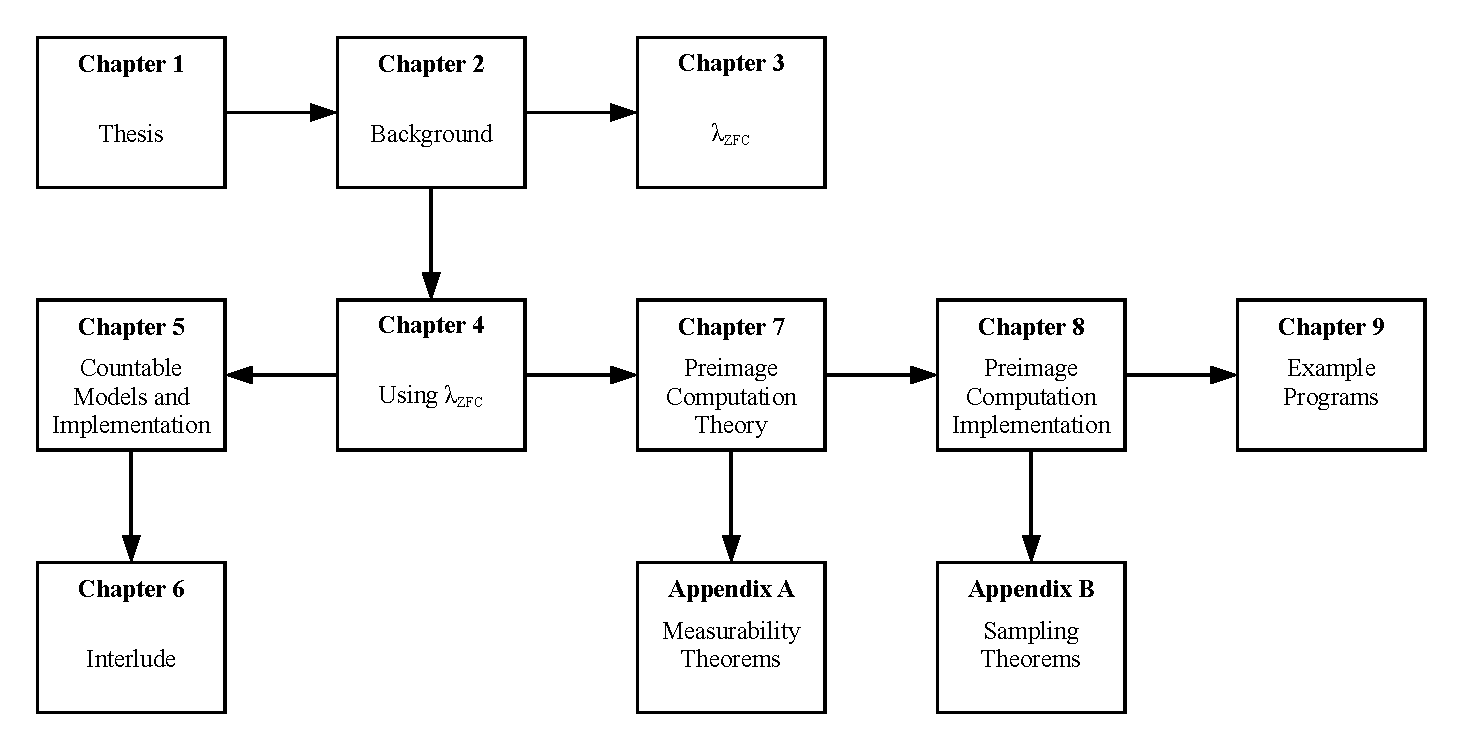
\includegraphics[width=\textwidth]{figures/reading-graph}
\caption[A transition system for reading this dissertation]{A transition system showing possible paths through this dissertation.}
\label{fig:reading-graph}
\end{figure*}

In principle, answers to questions such as ``Which chapters should I read if I am only interested in implementations of probabilistic languages with conditioning and recursion?'' can be answered using a dependency graph.
However, the graph would be a mess of arrows: for example, everything after Chapter~\ref{ch:background} (Background) depends on Chapter~\ref{ch:background}; similarly for Chapter~\ref{ch:using-lambda-zfc} (Using \lzfclang).
\figref{fig:reading-graph} shows an alternative: a transition system on chapters for which following any path (with backtracking permitted) guarantees a reader will not miss out on prerequisites.

Chapter~\ref{ch:background} gives the necessary background in Bayesian practice and functional programming theory, and motivates using measure theory.

The two semantics mentioned in the preceeding section transform programs into $\lambda$-calculus terms.
This target language has three requirements that are unusual for a $\lambda$-calculus: it must be able to represent infinite objects and operations on them, it must have nonterminating programs, and measure-theoretic theorems must apply directly to its terms.
Before this work, such a $\lambda$-calculus did not exist.
Chapter~\ref{ch:lambda-zfc} defines one, \lzfclang, with the precision necessary to carry out proofs with it.

While this precision is necessary for doing the rest of our work and verifying it, such precision is not necessary for understanding it.
Readers who are not verifying our work may therefore skip from Chapter~\ref{ch:background} to Chapter~\ref{ch:using-lambda-zfc}, which gives an overview of \lzfclang and its relationship with contemporary mathematics, gives examples of use, and defines some common terminology and functions.

Chapter~\ref{ch:countable-models} defines a semantics for Bayesian notation restricted to countable probability distributions and finitely many statements.
Chapter~\ref{ch:interlude} explains why its specific way of transforming notation into models does not extend easily to theories with recursion, which motivates a slight change in tactics.

Following the new tactics, Chapter~\ref{ch:preimage1} defines a semantics for a probabilistic language with uncountable distributions, recursion, and arbitrary probabilistic conditions.
Chapter~\ref{ch:preimage2} gives details that should be common to all implementations, and details specific to ours.

Appendix~\ref{ch:measurability} contains proofs of theorems critical to correctness, but whose inclusion in Chapter~\ref{ch:preimage1} would interrupt the narrative flow too much for readers unfamiliar with measure theory.
Appendix~\ref{ch:sampling-algorithm-proofs} is similar, but contains proofs of theorems from Chapter~\ref{ch:preimage2}.
While familiarity with measure theory is helpful while reading these two chapters, it is not strictly necessary: both explain the necessary concepts, and import enough definitions and lemmas from other sources to verify the proofs.
